\section{Le Méta-Modèle \kwentity{}}\label{sub:ent}


Le méta-modèle \kwentity{} représente une couche \guim{métier}. Il permet notamment de modéliser la persistance des données, ainsi que les relations entres elles. La figure \ref{fig:ent}  montre le méta-modèle \kwentity{} simplifié.

\begin{figure}[h]
  \centering
  
\includegraphics[scale=.4]{img/Entity.eps}
  \caption{Méta-modèle Entity}
  \label{fig:ent}
\end{figure}

Chaque block se compose de plusieurs Entity. Chacune d'elles possède un ou plusieurs attributs, et peut référencer d'autres Entity. Un attribut est caractérisé par un type, une multiplicité et une valeur. Chaque élément du modèle peut également inclure un ensemble de méta-données.

\subsection{Conception du modèle}

Nous avons employé la simple démarche suivante : pour chaque type de donnée susceptible d'être utilisée par notre application, on modélise une entité ainsi que l'ensemble de ses attributs. 
\kwplay{} utilise des mécanismes d'annotation au sein de ses modèles. Ces annotations permettent notamment de donner des contraintes à des attributs. Nous avons facilement pris en compte ce concept en utilisant les méta-données qu'il est possible d'intégrer au modèle d'un \verb+Attribut+.

Nous avons élaboré un modèle d'\kwentity de notre application conformément au Méta-Modèle que nous avons décris précédement. Ce modèle est illustré par la figure \ref{fig:entMod} ci-dessous.

\begin{figure}[h]
  \centering
  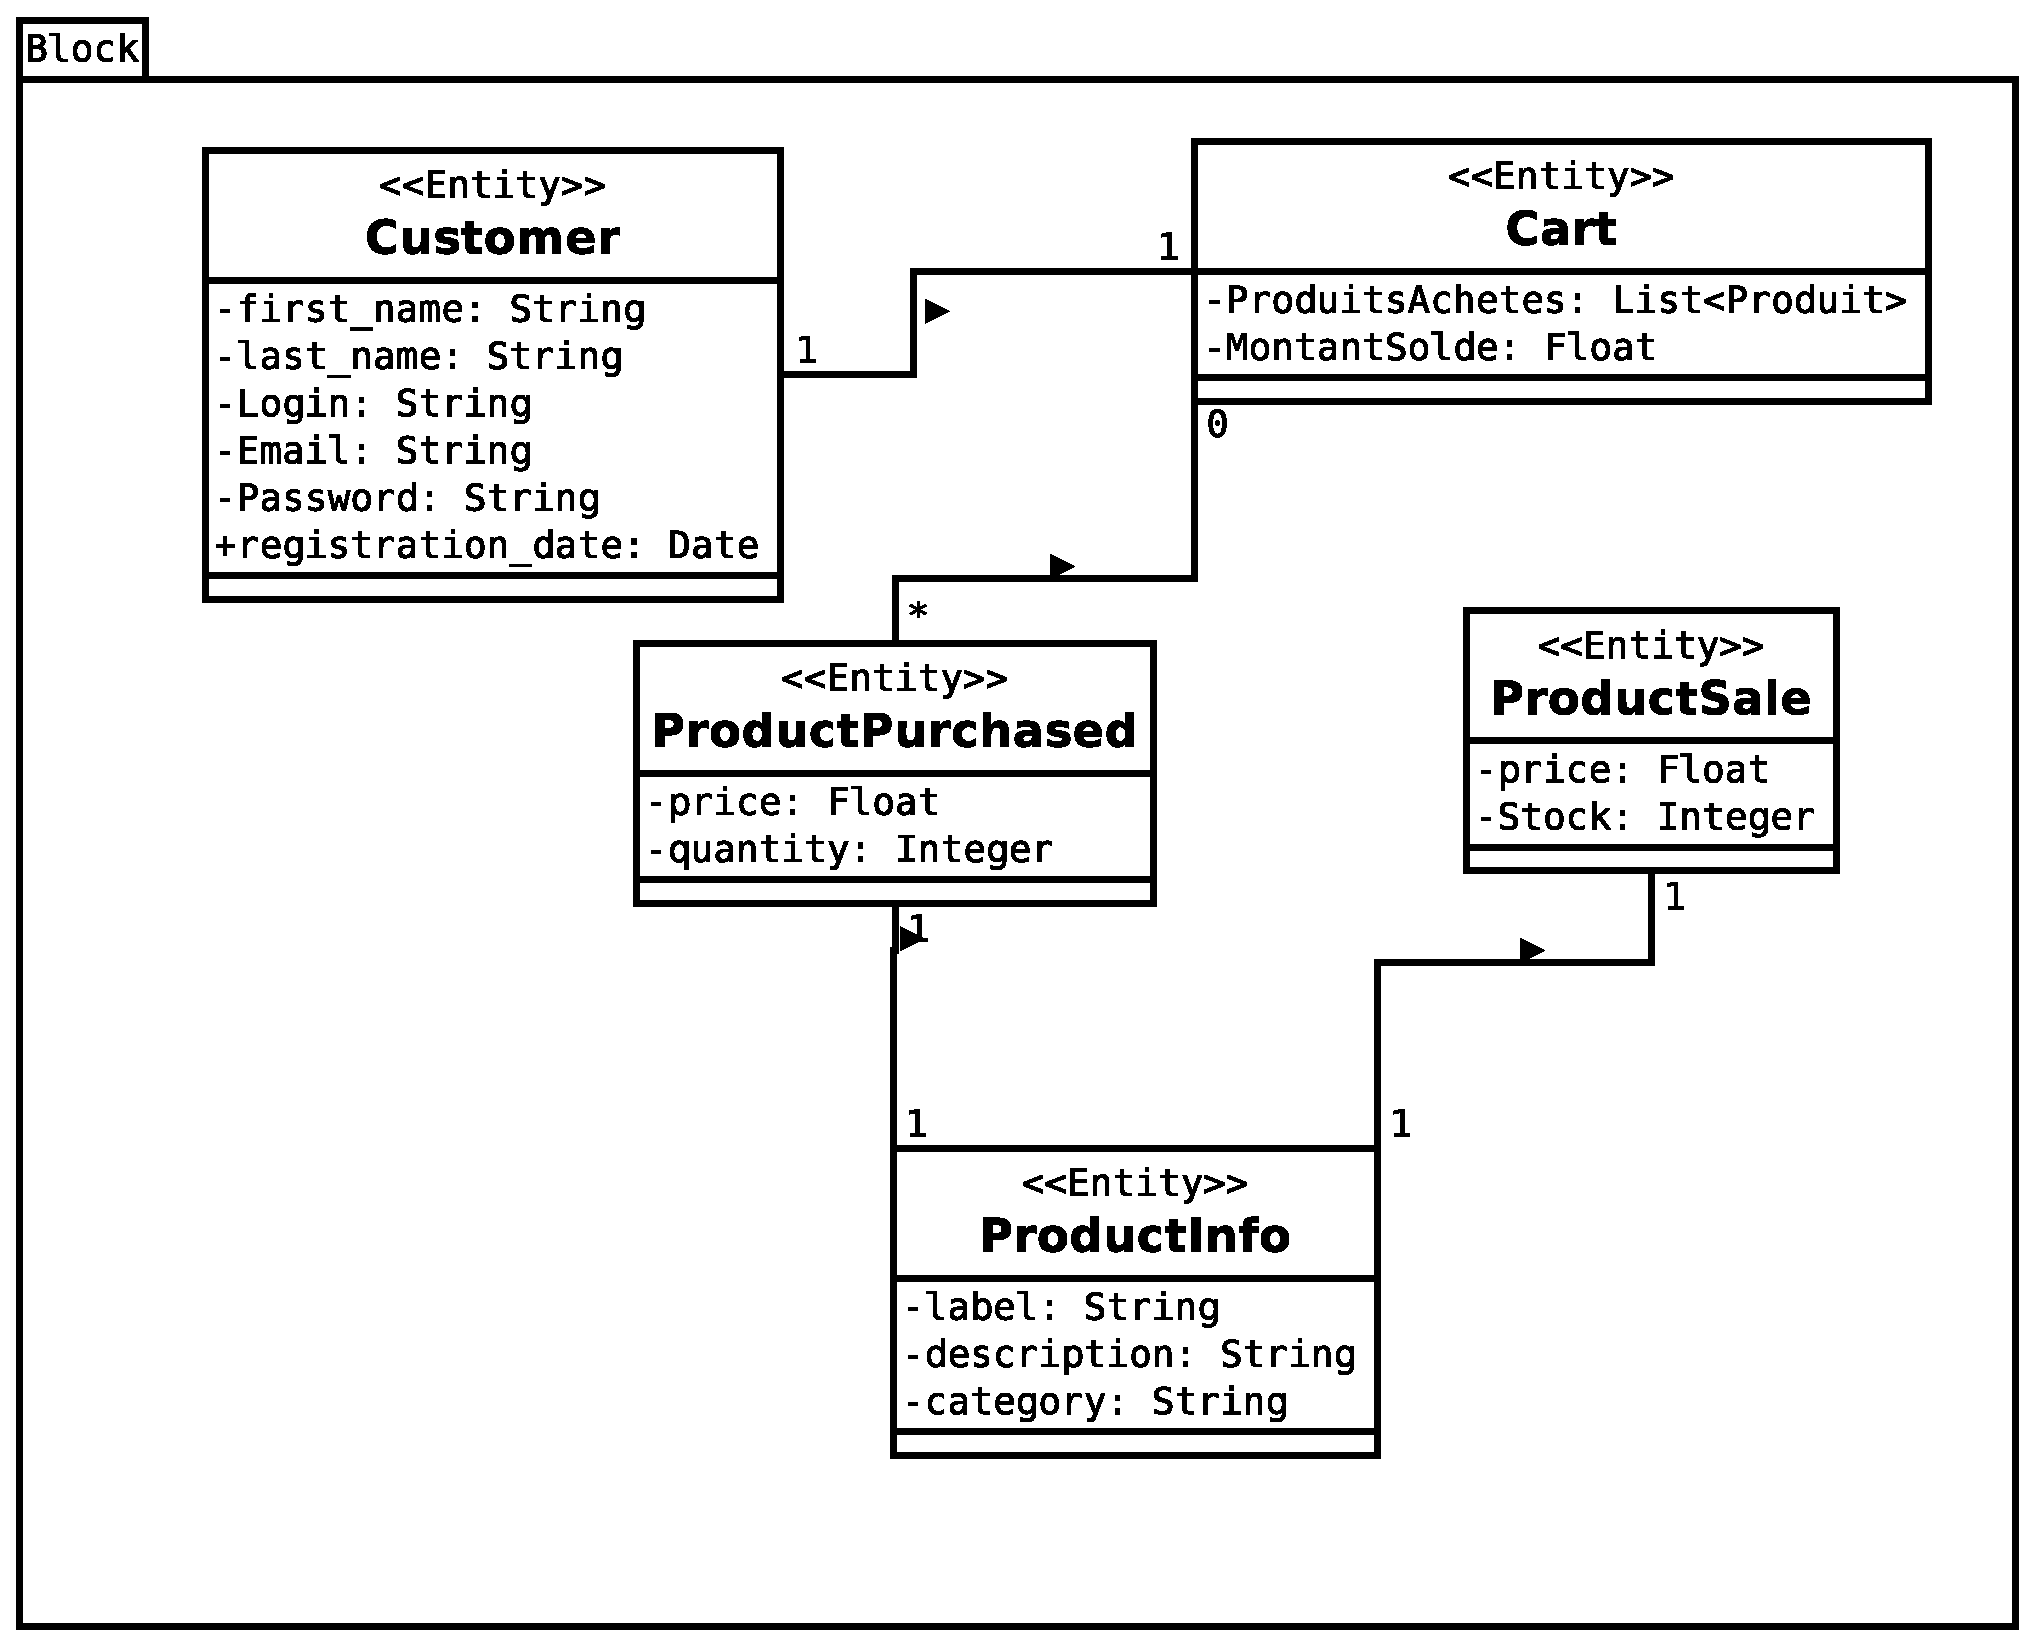
\includegraphics[scale=.4]{img/Entitymodel.eps}
  \caption{modèle Entity de l'application}
  \label{fig:entMod}
\end{figure}

Nous avons représenté un seul block dans notre modèle d'\kwentity{} qui va regrouper les \kwentity{} suivantes :  

\begin{itemize}
  \item[\textbullet] \textbf{Customer} :  client qui va faire l'achat sur la plate-forme.
  \item[\textbullet] \textbf{ProductSale} : les produits mis en vente.
  \item[\textbullet] \textbf{ProductPurchased} : les produits achetés par un client.
  \item[\textbullet] \textbf{ProductInfo} : contient les informations d'un produit.
  \item[\textbullet] \textbf{Cart} : panier virtuel du client.
\end{itemize}

\subsection{Génération du code \kwentity{}}

L'étape de construction des Générateurs de Code pour le Modèle \kwentity{} a été relativement simple : Pour chaque \kwentity{} contenue dans le Modèle, on génère une simple classe Java portant le nom de ladite Entité, puis on liste l'ensemble de ses attributs (types et propriétés). Ainsi, l'ORM \kwebean{} (intégré à \kwplay{}) interprétera simplement ces classes comme étant des données à stocker dans une Base.


%% \fbox{\parbox{\textwidth}{
%% [template public generateElement(myBlock : Block)]   // création du template.\newline
%% [for( myEntity : Entity | myBlock.entities)] //parcours des Entity. \newline
%% [file (myEntity.name + g-name-suffix() + '.java', false, 'UTF-8')] //création d'un fichier.\newline
%% [for(myEntity.attributes)] // parcours de tout les attributs. 
%% 	[comment Call the file block in 'attributes' /]\newline
%% 	[ generateAttribute() /] // appel d'un autre template qui affiche les attributs.\newline
%% [/for]
%% }}



% LocalWords:  Entity framework Model
